\section{Веб-приложение пациента}\label{sec:-211}

В эту часть веб приложения можно попасть из той же страницы авторизации только при использовании данных авторизации пациента.
Оно повторяет функционал Android-приложения.

\subsection{Главная страница}\label{subsec:-212}
При авторизации мы попадаем на главную страницу с опросами.
(См.\ рис. \ref{fig:figure53})
На ней представлены все возможные опросы для данного пациента.
Если уже прошло нужное время и пациенту снова нужно пройти опрос, кнопка прохождения активируется.
\begin{figure}[htbp]
    \centering
    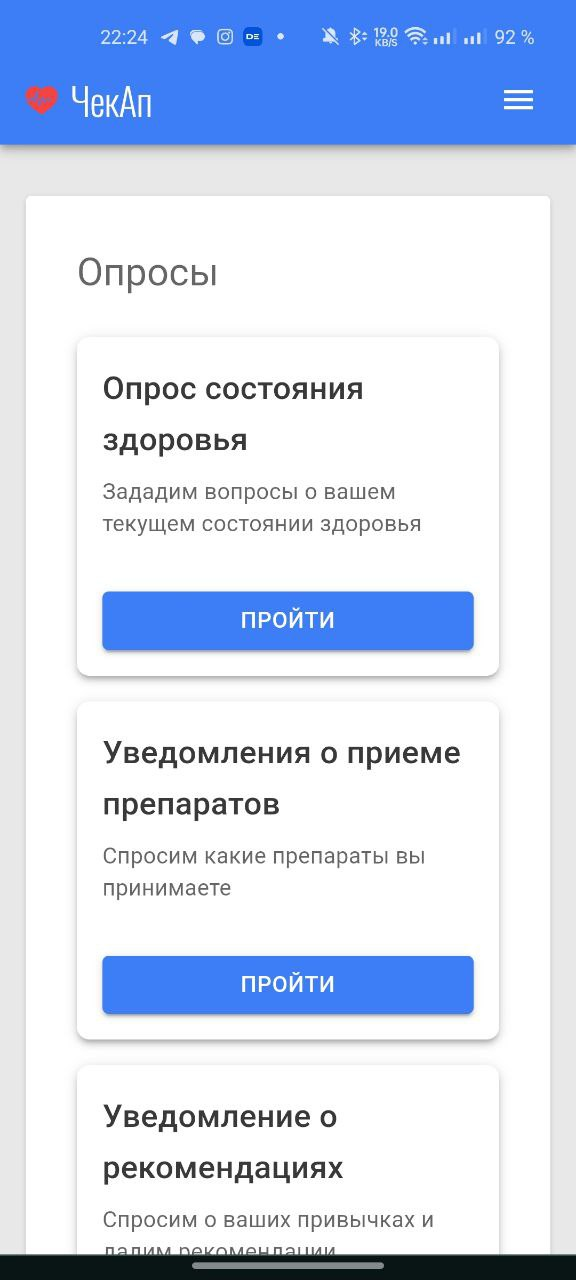
\includegraphics[height=\dimexpr\textheight/3\relax]{images/screenshots/main_page_patient}
    \caption{Главная страница пациента.}
    \label{fig:figure53}
\end{figure}

\subsection{Прохождения опроса}\label{subsec:-213}
Здесь представлен пример одного вопроса при прохождении опроса пациентом.
Здесь можно выбрать один вариант ответа (см.\ рис. \ref{fig:figure54}) или несколько вариантов ответов (см.\ рис. \ref{fig:figure56}).
После окончания опроса пациенту показывается экран успешности и предложение вернуться на главную страницу (см.\ рис. \ref{fig:figure57}).

\begin{figure}[htbp]
    \centering
    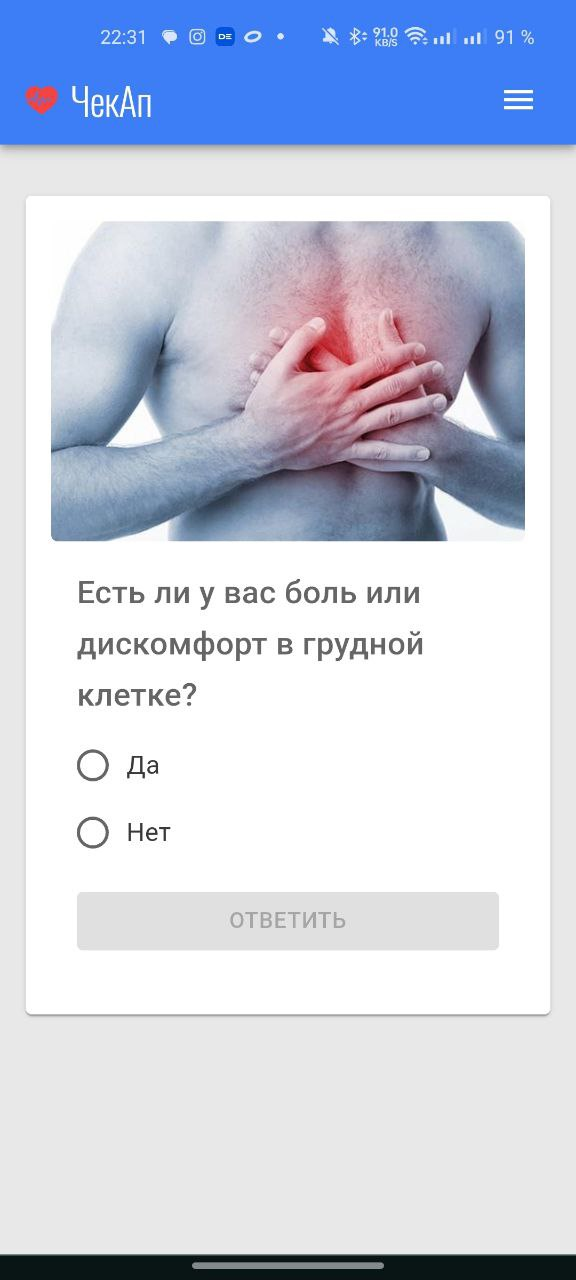
\includegraphics[height=\dimexpr\textheight/3\relax]{images/screenshots/process_inquirer}
    \caption{Пример вопроса в опроснике с одним вариантом ответа.}
    \label{fig:figure54}
\end{figure}

\begin{figure}[htbp]
    \centering
    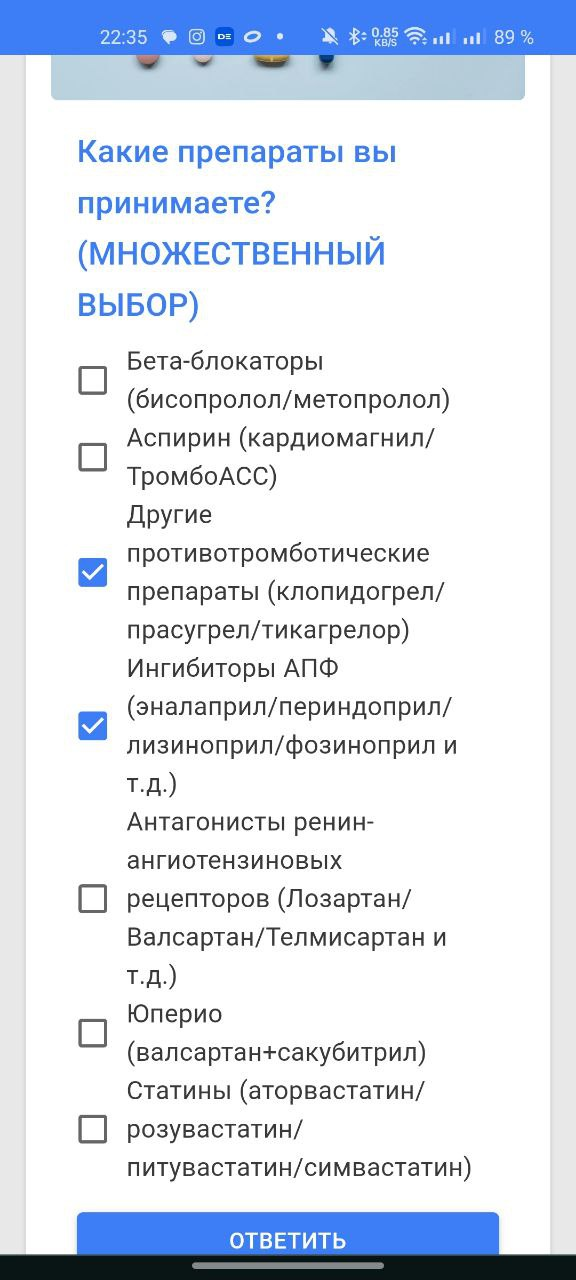
\includegraphics[height=\dimexpr\textheight/3\relax]{images/screenshots/process_inquirer_multi}
    \caption{Пример вопроса в опроснике с несколькими вариантами ответов.}
    \label{fig:figure56}
\end{figure}

\begin{figure}[htbp]
    \centering
    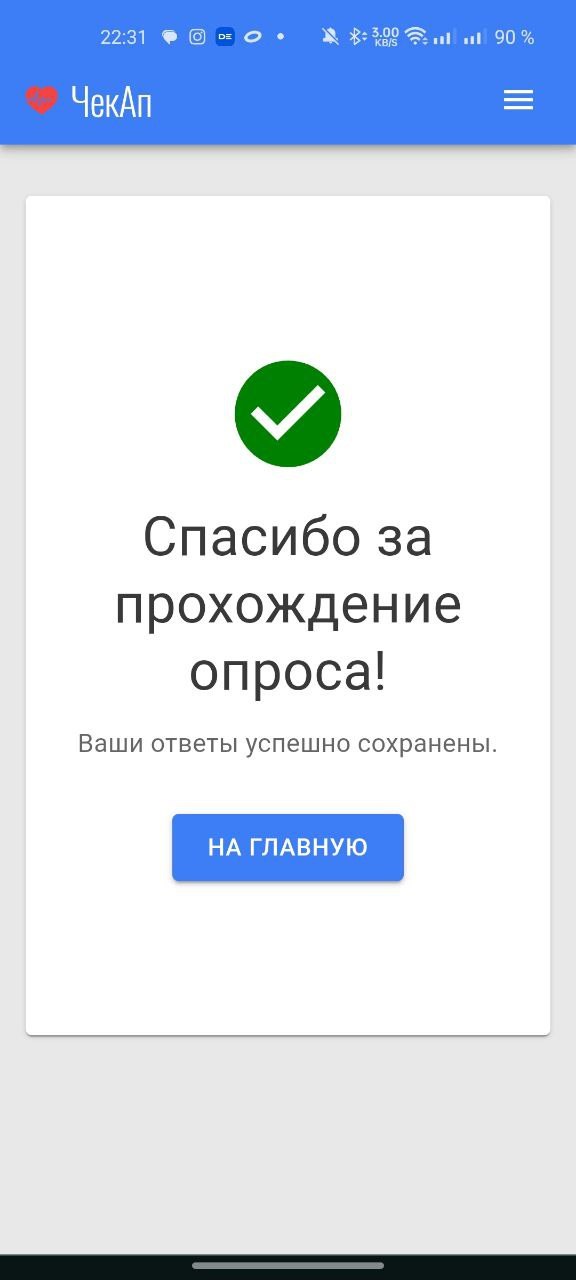
\includegraphics[height=\dimexpr\textheight/3\relax]{images/screenshots/inquierer_success}
    \caption{Успешное прохождение.}
    \label{fig:figure57}
\end{figure}

\subsection{Меню}\label{subsec:-214}
В мобильной версии функции хедера веб-приложения переходят в меню.
(Cм.\ рис. \ref{fig:figure58})
Его можно открыть при нажатии на появившуюся кнопку \("\)гамбургер\("\) в хедере.
В нем есть та же информация и функционал, что в обычной версии.
Пациент с его помощью может прервать опрос, перейдя на главную страницу

\begin{figure}[htbp]
    \centering
    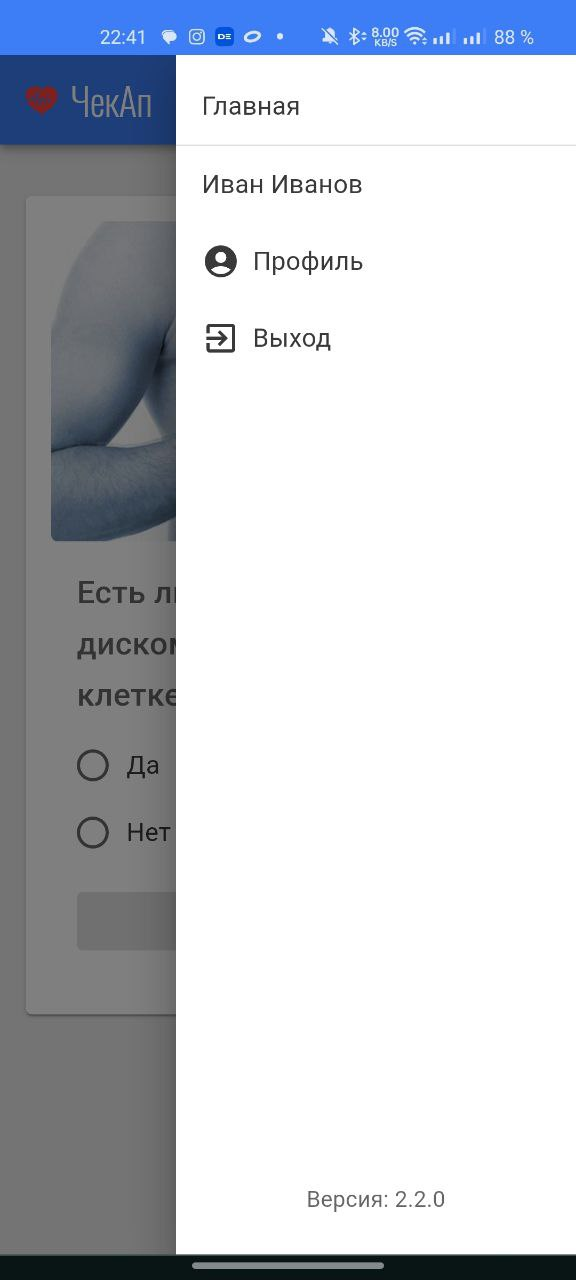
\includegraphics[height=\dimexpr\textheight/3\relax]{images/screenshots/menu_mobile}
    \caption{Меню мобильной версии приложения.}
    \label{fig:figure58}
\end{figure}






